\documentclass[sigconf]{acmart}

\usepackage[utf8]{inputenc}

\usepackage[lofdepth,lotdepth]{subfig}
\def\subfloatautorefname{Subfigure}

\usepackage{listings}
\usepackage{color}
\definecolor{mediumgray}{rgb}{0.3, 0.4, 0.4}
\definecolor{mediumblue}{rgb}{0.0, 0.0, 0.8}
\definecolor{forestgreen}{rgb}{0.13, 0.55, 0.13}
\definecolor{darkviolet}{rgb}{0.58, 0.0, 0.83}
\definecolor{royalblue}{rgb}{0.25, 0.41, 0.88}
\definecolor{crimson}{rgb}{0.86, 0.8, 0.24}

\lstdefinelanguage{JavaScript}{
  morekeywords=[1]{break, continue, delete, else, for, function, if, in,
    new, return, this, typeof, var, void, while, with},
  % Literals, primitive types, and reference types.
  morekeywords=[2]{false, null, true, boolean, number, undefined,
    Array, Boolean, Date, Math, Number, String, Object},
  % Built-ins.
  morekeywords=[3]{eval, parseInt, parseFloat, escape, unescape},
  sensitive,
  morecomment=[s]{/*}{*/},
  morecomment=[l]//,
  morecomment=[s]{/**}{*/}, % JavaDoc style comments
  morestring=[b]',
    morestring=[b]`,
  morestring=[b]"
}[keywords, comments, strings]
\lstdefinelanguage[ECMAScript2015]{JavaScript}[]{JavaScript}{
  morekeywords=[1]{await, async, case, catch, class, const, default, do,
    enum, export, extends, finally, from, implements, import, instanceof,
    let, static, super, switch, throw, try},
  morestring=[b]` % Interpolation strings.
}

\lstdefinestyle{JSES6Base}{
  backgroundcolor=\color{white},
  basicstyle=\ttfamily,
  basicstyle=\small,
  breakatwhitespace=false,
  breaklines=false,
  captionpos=b,
  columns=fullflexible,
  commentstyle=\color{mediumgray}\upshape,
  emph={},
  emphstyle=\color{crimson},
  extendedchars=true,  % requires inputenc
  fontadjust=true,
  frame=single,
  identifierstyle=\color{black},
  keepspaces=true,
  keywordstyle=\color{mediumblue},
  keywordstyle={[2]\color{darkviolet}},
  keywordstyle={[3]\color{royalblue}},
  numbers=left,
  numbersep=5pt,
  numberstyle=\tiny\color{black},
  rulecolor=\color{black},
  showlines=true,
  showspaces=false,
  showstringspaces=false,
  showtabs=false,
  stringstyle=\color{forestgreen},
  tabsize=2,
  title=\lstname,
  upquote=true  % requires textcomp
}

\lstdefinestyle{JavaScript}{
  language=JavaScript,
  style=JSES6Base
}

\lstdefinestyle{ES6}{
  language=ES6,
  style=JSES6Base
}

\setcopyright{}
\copyrightyear{2021. Licensed under a Creative Commons Attribution 4.0 International license.}
\acmYear{}
\acmConference{Thomas Steiner}
\acmBooktitle{François Beaufort}
\acmPrice{}
\acmDOI{}
\acmISBN{}

\settopmatter{printacmref=false}

\begin{document}

\title{Accessing \textsc{hid} Devices on the Web With the Web\textsc{hid} \textsc{api}}
\subtitle{How to play the Chrome Dino Game by Jumping With a Nintendo Joy-Con Controller in One's Pocket}

\author{Thomas Steiner}
\email{tomac@google.com}
\affiliation{%
  \institution{Google Germany GmbH}
  \streetaddress{ABC-Str. 19}
  \city{Hamburg}
  \postcode{20354}
  \country{Germany}
}

\author{François Beaufort}
\email{fbeaufort@google.com}
\affiliation{%
  \institution{Google France \textsc{sarl}}
  \streetaddress{8 Rue de Londres}
  \city{Paris}
  \postcode{75009}
  \country{France}
}

\renewcommand{\shortauthors}{}

\begin{abstract}
In this demonstration, we show how special hardware like Nintendo Joy-Con controllers
can be made accessible from the Web through the new Web\textsc{hid} \textsc{api}.
This novel technology proposal allows developers to write Web drivers in pure JavaScript
that talk to Human Interface Device (\textsc{hid}) devices via the \textsc{hid} protocol.
One such example of a driver has been realized in the project Joy-Con-Web\textsc{hid},
which allows for fun pastimes like playing the Google Chrome browser's
offline dinosaur game by jumping.
This works thanks to the accelerometers built into Joy-Con controllers
whose signals are read out by the driver and used to control the game
character in the browser. A~video of the experience is available.
\end{abstract}

\begin{CCSXML}
<ccs2012>
<concept>
<concept_id>10002951.10003260.10003282</concept_id>
<concept_desc>Information systems~Web applications</concept_desc>
<concept_significance>500</concept_significance>
</concept>
<concept>
<concept_id>10002951.10003260.10003300.10003302</concept_id>
<concept_desc>Information systems~Browsers</concept_desc>
<concept_significance>500</concept_significance>
</concept>
</ccs2012>
\end{CCSXML}

\ccsdesc[500]{Information systems~Web applications}
\ccsdesc[500]{Information systems~Browsers}

\keywords{Progressive Web Apps, Web \textsc{api}s, Web\textsc{hid}}

\maketitle

\section{Introduction and Background}

Universal Serial Bus (\textsc{usb}) is a communications architecture
that gives a personal computer (\textsc{pc}) the ability to interconnect
a~variety of devices using a simple four-wire cable.
These devices are broken into various device classes.
One of these classes is the Human Interface Device (\textsc{hid}) class.
The \textsc{hid} class consists primarily of devices that are used by humans
to control the operation of computer systems.
Typical examples of \textsc{hid} class devices include~\cite{hid01}:

\begin{enumerate}
  \item Keyboards and pointing devices---for example: standard mouse devices,
        trackballs, and joysticks.
  \item Front-panel controls---for example: knobs, switches, buttons, and sliders.
  \item Controls that might be found on devices such as telephones, \textsc{vcr}
        remote controls, games or simulation devices---for example: gloves,
        throttles, steering wheels, and rudder pedals.
  \item Devices that may not require human interaction but provide data in a~similar
        format to \textsc{hid} class devices---for example: bar-code readers, 
        thermometers, or voltmeters.
\end{enumerate}

The \textsc{hid} protocol was originally developed for \textsc{usb} devices,
but has since been implemented over many other protocols, including Bluetooth.
For the context of this demonstration, we focus on gamepad devices of the category (1)
that connect over Bluetooth.

\section{Related Work}

The Gamepad specification~\cite{gamepad20} defines a low-level interface
that represents gamepad devices and allows Web applications
to directly act on gamepad data.
Interfacing with external devices designed to control games has the potential
to become large and intractable if approached in full generality.
The authors of the specification explicitly chose to narrow the scope
to provide a useful subset of functionality that can be widely implemented and
that is broadly useful.
Specifically, they chose to only support the functionality required to support gamepads.
Support for gamepads requires two input types: buttons and axes.
Both buttons and axes are reported as analog values.
The authors deliberately excluded support for more complex devices that may also be used
in gaming contexts, including those that do motion or depth sensing,
video analysis, gesture recognition, \textit{etc.}
One such example are Nintendo's Joy-Con controllers
that contain gyroscopes and accelerometers.

\section{The Web\textsc{hid} \textsc{api}}

The Web\textsc{hid} \textsc{api}~\cite{webhid21} closes this gap by providing a~way
to implement device-specific logic in JavaScript.
This \textsc{https}-only \textsc{api} is asynchronous by design to prevent the website \textsc{ui}
from blocking when awaiting \textsc{hid} input.
This is important because \textsc{hid} data can be received at any time,
requiring a way to listen to it.
\textsc{hid} consists of two fundamental concepts: reports and report descriptors.
Reports are the data that is exchanged between a device and a~software client.
The report descriptor describes the format and meaning of data that the device supports.
A~report descriptor describes the binary format of reports supported by the device.
Applications and \textsc{hid} devices exchange binary data through three report types:

\begin{itemize}
  \item \textbf{Input report:}	Data that is sent from the device
    to the application (\textit{e.g.},\ a button is pressed.)
  \item \textbf{Output report:}	Data that is sent from the application
    to the device (\textit{e.g.},\ a request to turn on the keyboard backlight.)
  \item \textbf{Feature report:} Data that may be sent in either direction.
    The format is device-specific.
\end{itemize}

To open a \textsc{hid} connection, a \texttt{HIDDevice} object needs to be accessed.
This can either happen by prompting the user to select a device by calling
\texttt{navigator.hid.requestDevice()},
or by picking one from \texttt{navigator.hid.getDevices()},
which returns a list of devices the website has been granted access to previously.
The \texttt{navigator.hid.requestDevice()} function takes a mandatory parameter \texttt{filter}
used to match any device connected with a \textsc{usb} vendor identifier (\texttt{vendorId}),
a \textsc{usb} product identifier (\texttt{productId}),
a usage page value (\texttt{usagePage}), and a usage value (\texttt{usage})
that can be obtained from the \textsc{usb} \textsc{id}
Repository\footnote{\url{http://www.linux-usb.org/usb-ids.html}}
and the \textsc{hid} usage
tables\footnote{\url{https://usb.org/document-library/hid-usage-tables-12}} document.
\autoref{code:connect} shows how to connect to Joy-Con controllers.

\begin{lstlisting}[language=JavaScript, style=ES6, caption={Connecting to Nintendo Joy-Con controllers}, label={code:connect}]
// Feature detection to see if the API is supported.
if (!("hid" in navigator)) return;
// Filter on Nintendo Switch Joy-Cons.
const filters = [{
  vendorId: 0x057e, // Nintendo Co., Ltd
  productId: 0x2006 // Joy-Con Left
},{
  vendorId: 0x057e, // Nintendo Co., Ltd
  productId: 0x2007 // Joy-Con Right
}];
// Prompt the user to select a Joy-Con device.
const [device] = await navigator.hid.requestDevice({ filters });
\end{lstlisting}

Once the \textsc{hid} connection has been established, incoming input reports are handled
by listening to \texttt{"inputreport"} events from the device.
Those events contain the \textsc{hid} data as a
\texttt{DataView} object (\texttt{data}),
the \textsc{hid} device it belongs to (\texttt{device}),
and the 8-bit report \textsc{id} associated with the input report (\texttt{reportId}).
\autoref{code:input} shows how to detect button presses on Nintendo Joy-Con controllers.

\begin{lstlisting}[language=JavaScript, style=ES6, caption={Listening to Joy-Con controller input reports}, label={code:input}]
device.addEventListener("inputreport", event => {
  const { data, device, reportId } = event;
  // Handle only the Joy-Con Right device and a specific report ID.
  if ((device.productId !== 0x2007) && (reportId !== 0x3f)) return;
  const value = data.getUint8(0);
  if (value === 0) return;
  const buttons = { 1: "A", 2: "X", 4: "B", 8: "Y" };
  console.log(`Pressed button ${buttons[value]}.`);
});
\end{lstlisting}

\section{Security and Privacy}

The spec authors have designed and implemented the Web\textsc{hid} \textsc{api}
using the core principles defined in
Controlling Access to Powerful Web Platform Features~\cite{ng19},
including user control, transparency, and ergonomics.
The ability to use this \textsc{api} is primarily gated by a permission model
that grants access to only a single \textsc{hid} device at a time.
In response to a user prompt, the user must take active steps
to select a particular \textsc{hid} device.
More details about the security tradeoffs can be found in
the Security and Privacy Considerations section of the Web\textsc{hid} spec~\cite{hid01}.
Chromium---as the currently sole implementing engine with Chrome and Edge as example user-agents that ship this API---inspects
the usage of each top-level collection,
and if a top-level collection has a protected usage
(\textit{e.g.}\ generic keyboard, mouse), then a website won't be able to send and receive
any reports defined in that collection.
The full list of protected usages is publicly
available.\footnote{\url{http://goo.gle/hid-usage-and-page_cc}}
Security-sensitive \textsc{hid} devices
(such as \textsc{fido} \textsc{hid} authentication devices)
are blocked in Chrome.\footnote{\url{http://goo.gle/hid-blocklist_cc}}

\section{Demonstration}

We have implemented a Web\textsc{hid} driver for Nintendo Joy-Con controllers
that allows for full access to all of the controllers' buttons, axes,
motion actuators, accelerometers, and gyroscopes.
The project is available on GitHub.\footnote{\url{https://github.com/tomayac/joy-con-webhid}}
Figure~\ref{fig:webhid} shows the driver's demo, where the orientation of the controllers
in the hands of the user is reflected virtually on the screen. 
To demonstrate the practicability of the driver, we have adapted the Chrome offline dino game~\cite{dino18}
so that it can be played by jumping with a Joy-Con controller in one's pocket.
This game is likewise available on GitHub.\footnote{\url{https://github.com/tomayac/chrome-dino-webhid}}
A video of the experience can additionally be seen on
YouTube.\footnote{\url{https://www.youtube.com/watch?v=HuhQXXgDnCQ}}
Figure~\ref{fig:dino} shows one of the authors interact with the demonstration
by jumping.

\section{Conclusion}

The Web platform already supports input from many \textsc{hid} devices.
Keyboards, pointing devices, and gamepads are all typically implemented
using the \textsc{hid} protocol.
However, this support relies on the operating system's \textsc{hid} drivers
that transform \textsc{hid} input into high-level input \textsc{api}s.
Devices that are not supported by the host's \textsc{hid} drivers are
inaccessible to Web pages.
Providing access to \textsc{hid} devices through the Web platform
reduces installation requirements, particularly for devices that are
currently only supported through host-specific applications.
With our demonstration, we have motivated the existence of 
the Web\textsc{hid} \textsc{api} and proven its practicability.

\begin{figure}
  \centering
  \subfloat[][Demo of the driver]{
    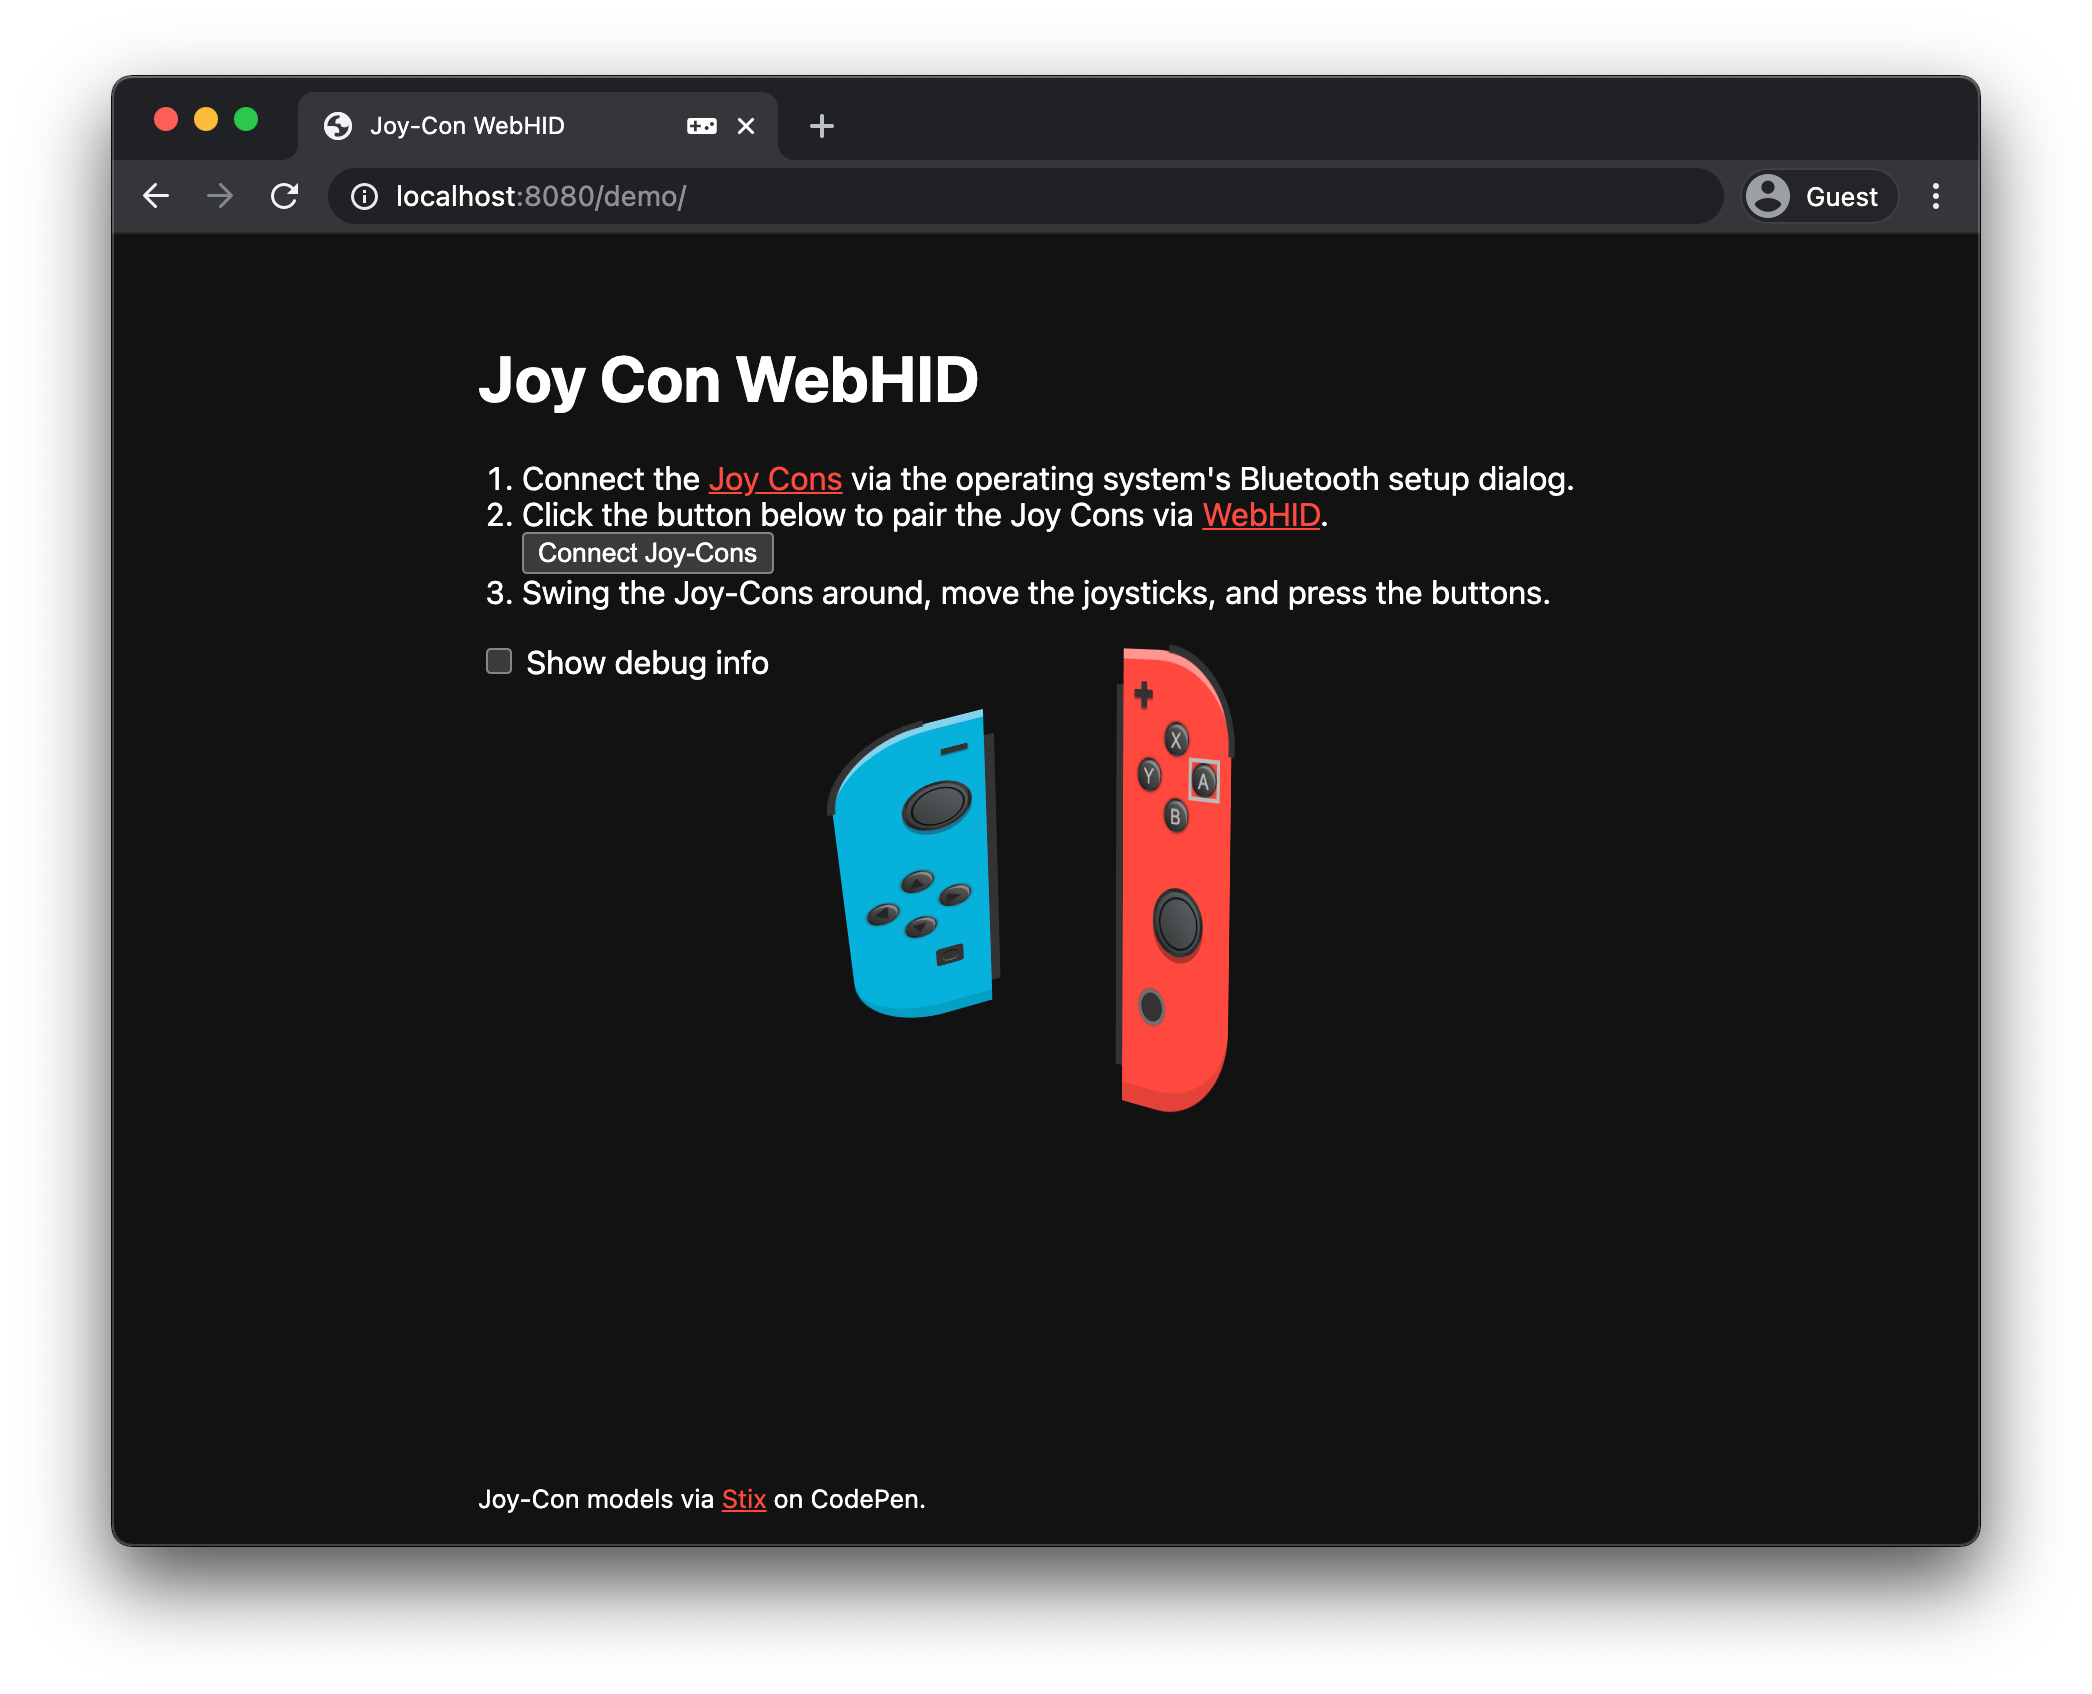
\includegraphics[width=0.372\columnwidth]{webhid.png}
    \label{fig:webhid}
  }
  \subfloat[][Playing by jumping]{
    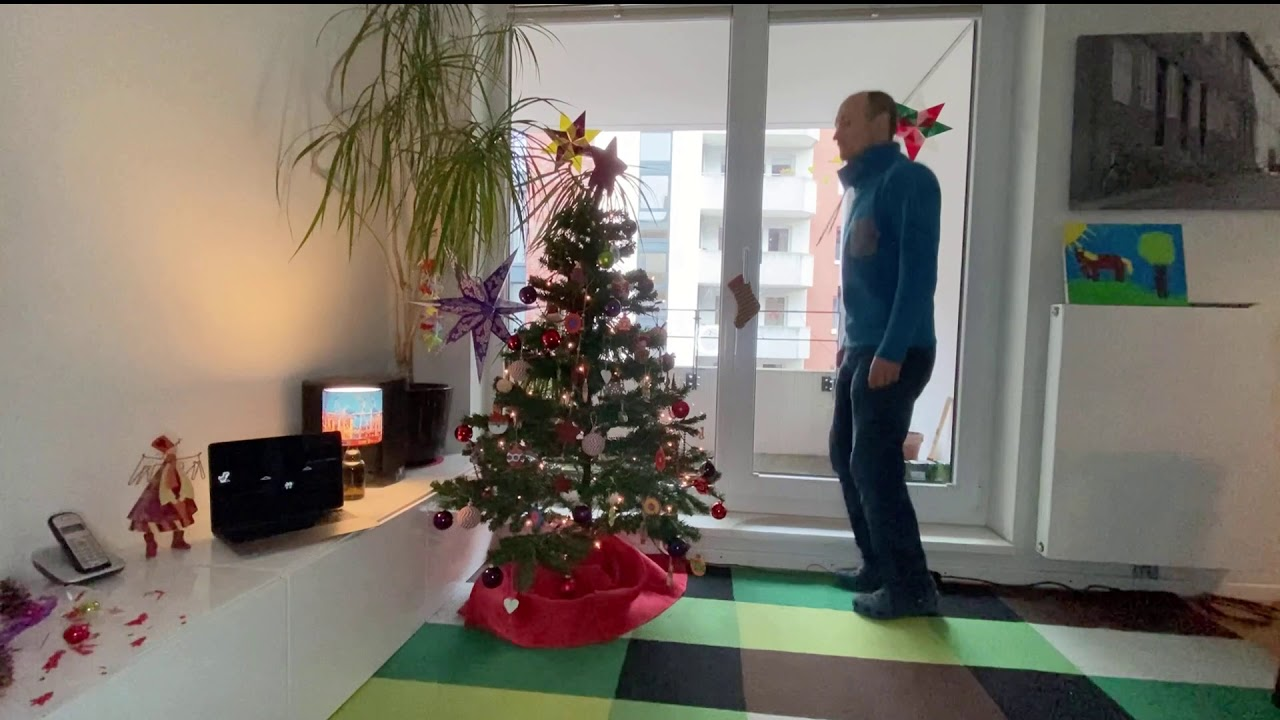
\includegraphics[width=0.58\columnwidth]{dino.jpg}
    \label{fig:dino}
  }
  \label{fig:double}
  \caption{Joy-Con Web\textsc{hid} and Chrome Dino Web\textsc{hid}}
\end{figure}

\bibliographystyle{ACM-Reference-Format}
\bibliography{webhid}

\end{document}
\endinput
